
\documentclass[12pt]{article}
\usepackage[letterpaper,textwidth=5.5in,right=0.6in,textheight=9in,left=0.6in,top=0.7in,bottom=0.7in]{geometry}

\usepackage{amsmath,amssymb}
\usepackage{graphicx}
\begin{document}
	\noindent 1.
	
	Let us consider the optimal coloring $\chi(G) = k$. Let us consider the folling Coloring classes $C_i = \{v \in V(G) | c(v) = i\}$. Let $k_i = \{C_1 \cup C_2 \cup ... \cup C_i\}$ for $1 \leq i \leq k_i$. Let $k_i$ be 0. Thus we can arrange the vertices such that $C_i = \{v_{k_{i-1}+1},v_{k_{-1}+2},...v_{k_i}\}$. Thus given this coloring, we will be able to cover the Graph with k colors since $1 \leq i \leq k$.
	
	\hfill $\blacksquare$
	
	\noindent2.Let us prove $\chi(G) \leq \Delta(G) + 1$ using induction on graph $G$ that has fixed $|V(G)| = n$ and $\Delta(G) = k$.\\
	
	\noindent Base case:
	
	We have $V(G) = n$ and $\Delta(G) = 0$. In other words, $\forall u \in V(G), \forall v \in V(G) , \nexists (u,v) \in E(G)$. Therefore, one color is sufficient for coloring this graph. Thus we have $\chi(G) = 1 \leq 0+1 \leq \Delta(G) + 1$. Therefore the base case holds.\\
	
	 \noindent Inductive Hypothesis: Assume $\chi(G) \leq \Delta(G) + 1$ holds for graph $G$ which has $|V(G)| = n$ and $\Delta(G) = k -1$.\\
	 
	 \noindent Inductive Step: Assume the inductive hypothesis holds and prove I.H. holds for case $V(G) = n$ and $\Delta(G) = k$ holds.
	 
	 We connect one more vertex $v_1$ to the vertex that has the maximum degree $v_2$ in graph $G$ to construct a $G'$ such that $V(G') = n$ and $\Delta(G') = k$. Consider 3 exhaustive cases:\\
	 
	 \noindent 1. $c(v_1) \neq c(v_2)$.
	 
	 In this case, We do not need to modify anything, and we have $\chi(G') = \chi(G) \leq k+1 \leq \Delta(G) + 1$\\
	 
	 \noindent 2. $c(v_1) = c(v_2)$ and $\exists v_j \in V(G'-v_1 - v_2)$ such that $c(v_j) = c(v_1) = c(v_2)$.
	 
	 In this case, we replace $c(v_1)$ with a new color so that $\nexists v_j \in V(G' - v_1 -v_2)$ such that $v_j = v_1$. Thus we have $\chi(G') = \chi(G) + 1 \leq ((k-1)+1)+1 \leq k+1 \leq \Delta(G')+1$.\\
	 
	 \noindent 3. $c(v_1) = c(v_2)$ and $\nexists v_j \in V(G'-v_1 - v_2)$ such that $c(v_j) = c(v_1) = c(v_2)$.
	 
	 In this case, we replace $c(v_1)$ with a new color so that $\nexists v_j \in N(v_1)$ such that $c(v_j) = c(v_1)$ and $c(v_1) \neq c(v_2)$. Thus we have $\chi(G') = \chi(G) + 1 \leq ((k-1)+1)+1 \leq k+1 \leq \Delta(G')+1$.
	 
	 \noindent Thus we have shown the Inductive step holds for all cases. Combining with the base case, we have proved $\chi(G) \leq \Delta(G) + 1$.
	 
	 	\hfill $\blacksquare$
	 	
	\noindent 3. To construct $G'$ with $\chi(G') = 2$ from a graph $G$ that contains no odd cycles, we first rearrange the vertices in $G$ to form two vertex sets $X$ and $Y$ where $\forall u \in X, \forall v \in X, \nexists (u,v) \in E(G)$ and $\forall u \in Y, \forall v \in Y, \nexists (u,v) \in E(G)$. Note here the rearrangement is feasible since $G$ contains no odd cycles $\implies$ $G$ is bipartite. Then we add the vertex set $U = \{u_1,...,u_{||X|-|Y||}\}$ to the set with smaller size between $X$ and $Y$.
	After adding the set, we have $|X| = |Y|$. Then $\forall u \in X$, we add an edge between u and all vertices $v \in Y$ to construct $G'$. Therefore $\forall v \in G', d(v) \geq \dfrac{|V(G')|-1}{2}$ since every vertex is connected to $\dfrac{|V(G')|}{2}$ vertices in the other part of the bipartite graph. $G'$ is still 2 colorable since it is still a bipartite graph, and all bipartite graph are $2$ colorable.
	
	\hfill $\blacksquare$
	
	\noindent 4. Based on the previous 2 problems, we can claim $\chi(G) \leq \Delta(G) + 1$ for a general graph. A connected graph always $k-colorable$ where $k \geq 2$.
	
	\hfill $\blacksquare$
	
	\noindent 5. In order to prove the chromatic polynomial for $K_n$ is $\chi(K_n, k) = k(k-1)\ldots(k-n+1)$, we use induction on the number of vertices of $K_n$.\\
	
	\noindent Base Case:
	
	For non-trivial graph $K_1$ with $|V(G)| = 1$, we know it can be colored with k colors. Thus $\chi(G) = k..(k-1+1) = k(k-1)\ldots(k-n+1)$. Therefore the base case holds.\\
	
	\noindent Inductive Step:
	
	Assume graph $K_n$ has chromatic polynomial $\chi(K_n, k) = k(k-1)\ldots(k-n+1)$. Prove graph $K_{n+1}$ has chromatic polynomial $\chi(K_{n+1}, k) = k(k-1)\ldots(k-n+1)k(n-1)$.
	
	To construct graph $K_{n+1}$, we add $v_n$ vertex to the graph $K_n$ and $\forall v_i \in V(K_n-v_n)$, we connect $v_i$ with $v_n$. Since $k_n$ is a clique, we have used $n$ colors and thus $v_n$ has $(k-n)$ color options. From our Inductive hypothsis we know $\chi(K_n, k) = k(k-1)\ldots(k-n+1)$. Since $v_n$ has $(k-n)$ color options, we know $K_{n+1}$ has chromatic polynomial $\chi(K_{n+1}, k) = k(k-1)\ldots(k-n+1)k(n-1)$. Therefore the Inductive step holds.
	
	Since both the base case and inductive step hold, we have proved $\chi(K_n, k) = k(k-1)\ldots(k-n+1)$.
	
		\hfill $\blacksquare$
		
	\noindent 6. Claim: $2 \leq \chi(G) \leq 3$.

	For the lowerbound: A graph with more than 1 vertex is at least 2-colorable. For the upperbound: Consider the cut vertex $v_c \in V(G)$ such that the number of components in $G-v_c$ is $4$. Since $G$ is biconnected, we know $d(v_c) = 4$ and $v_c$ is in 4 different cycles since every biconnected graph of $G$ is ismporphic to $C_n$. We first give $v_c$ color $c_1$, then we can color $C_n$ with $3$ colors if $n$ is odd and $2$ colors if $n$ is even. Thus we can color all the cycles with $\max{3,2}-1 = 2$ extra colors. We substract one since $v_c$ is in all the cycles and we have already counted that color. Since the coloring in one cycle will not affect the coloring in another cycle (they only have one common vertex $v_c$), we can color all the vertices with $2+1(\text{the color for }v_c)=3$ colors. Since the bound holds for the cut vertex $v_c$ that results in the maximum number of components in $G-v_c$, it holds for all the other cut vertices. Thus we have $\chi(G) \leq 3$.
	
	\hfill $\blacksquare$
	
	\noindent 7. In order to prove  $G$ is $k$-color-critical for $\chi(G) = k = 3$ if and only if $G$ is an odd cycle, we need to prove (i).  $G$ is $k$-color-critical for $\chi(G) = k = 3$ $\implies$ $G$ is an odd cycle. (ii). $G$ is an odd cycle $\implies$ $G$ is $k$-color-critical for $\chi(G) = k = 3$.
	
	(i). If $G$ is $k$-color-critical for $\chi(G) = k = 3$, then $G$ is not 2 colorable. Therefore $G$ must contain an odd cycle. Let $C$ be the smallest odd cycle of graph $G$. If $G \neq C$, then $C$ is a proper induced subgraph with $\chi(C) = \chi(G) = 3$. Thus it must be the case $G = C$ since $G$ is 3-color critical. Otherwise we would have a contradiction. Since $G$ is $3$-color critical and $G = C$, we can conclude $G$ is $k$-color-critical for $\chi(G) = k = 3$ $\implies$ $G$ is an odd cycle.
	
	(ii). If $G$ is an odd cycle, then $G$ is $3$ colorable and is not $2$ colorable. Removing any vertex in $G$ breaks the cycle and thus become 2 colorable. Thus we can conclude $G$ is an odd cycle $\implies$ $G$ is $k$-color-critical for $\chi(G) = k = 3$.
	
	Since we have proved the statement holds for both direction, we can prove  $G$ is $k$-color-critical for $\chi(G) = k = 3$ if and only if $G$ is an odd cycle.
	
		\hfill $\blacksquare$
		
	\newpage
	
	\noindent 8.
	
	\begin{figure}[h]
		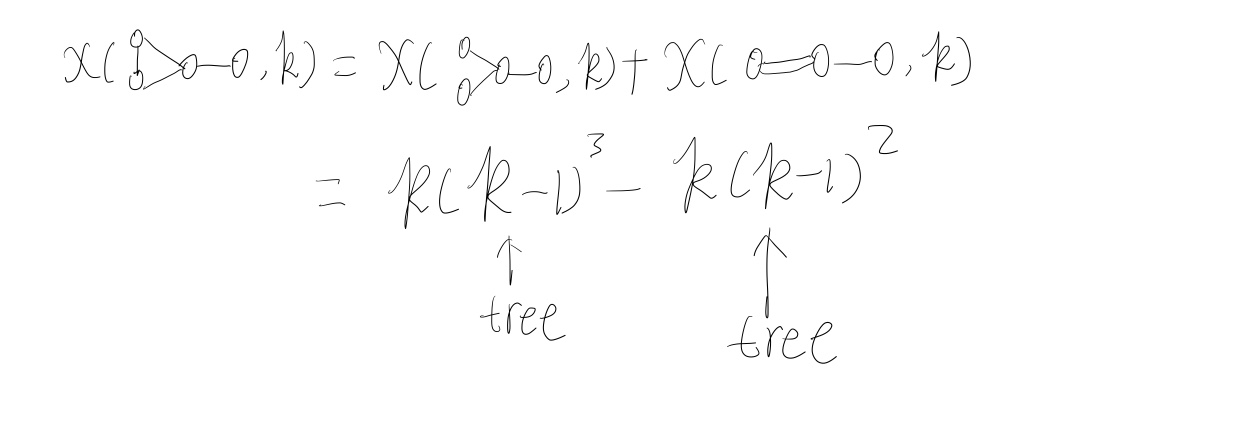
\includegraphics[scale = 0.4]{"C:/Users/Micha/OneDrive - Rensselaer Polytechnic Institute/Graph Theory/pictures/hw5-1.png"}\\
	\end{figure}
	In the second recurrence relation, the number of edges between two vertices does not matter.To determine the Chromatic number $\chi(G)$, we set $\chi(G,k) = k(k-1)^3-k(k-1)^2 > 0$. Thus we have $k>2$ (said by WolframAlpha). Therefore we have $\chi(G) = 3$.
	
	\noindent 9.
	
	\begin{figure}[h]
		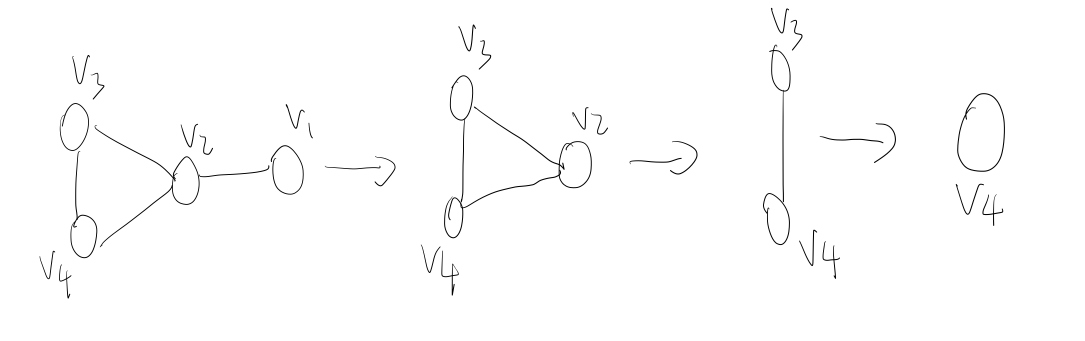
\includegraphics[scale = 0.6]{"C:/Users/Micha/OneDrive - Rensselaer Polytechnic Institute/Graph Theory/pictures/hw5-2.png"}\\
	\end{figure}
	The simplicial elimination ordering is $\{v_1,v_2,v_3,v_4\}$. Since G has a simplicial elimination odering, it is a chordal graph. Since G is a chordal graph, it is a perfect graph.\\
	\newpage
	\noindent 10.
		\begin{figure}[h]
		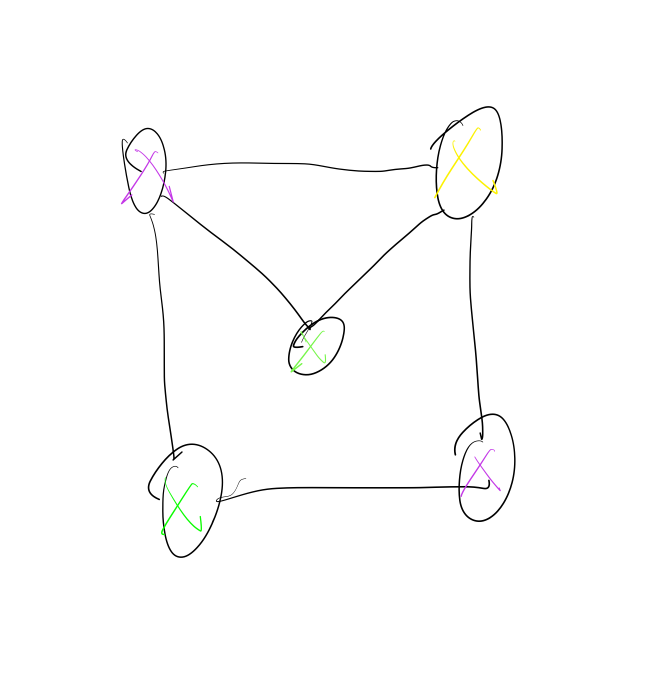
\includegraphics[scale = 0.6]{"C:/Users/Micha/OneDrive - Rensselaer Polytechnic Institute/Graph Theory/pictures/hw5-3.png"}\\
	\end{figure}

	As we can see, $\chi(G)= \omega(G) = 3$. Howeverk, there's a properly induced subgraph $k_3$ wihich has $\chi(k_3) = 3$ and $\omega(k_3)$. Thus $G$ is not perfect.
\end{document}